\documentclass[a4j]{jarticle}
\title{ファインマンダイヤグラムの書き方〜tikz-feynhand編〜}
\usepackage[dvipdfmx]{graphicx}
\usepackage{tikz}
\usepackage{tikz-feynhand}
\begin{document}
\maketitle

\section{ダイヤグラムを書くために}
ダイヤグラムを書く一つの方法が,feynmpパッケージを使う方法である.usepackageでfeynmpとする
http://osksn2.hep.sci.osaka-u.ac.jp/~taku/osx/feynmp/fmfsamples.pdf
この方法では,一つのtexファイルで一つのダイヤグラムを作ることしかできない上,いちいちmpostコマンドを実行しないといけないのが難点であるが,後述のtikz-feynhandでは不可能なバーテックスの表現や,行列グリーン関数なども表現可能なため,より複雑なダイヤグラムを書きたい時はこちらを推奨する.

ただとりあえずは,tikz-feynhandを用いることにする.これはtikzpicture環境の中にfeynhand環境を作ることでダイヤグラムをtikz感覚で作ってくれる.

\section{バーテックス}
頂点は,vertexコマンドで生成できる.これは普通のtikzとよく似ていて,
オプションとして
particle, dot, ringdot, squaredot, crossdot,
blob, ringblob, grayblob, NWblob, NEblob
の$10$個が用意されている.
\begin{figure}[htb]
\centering
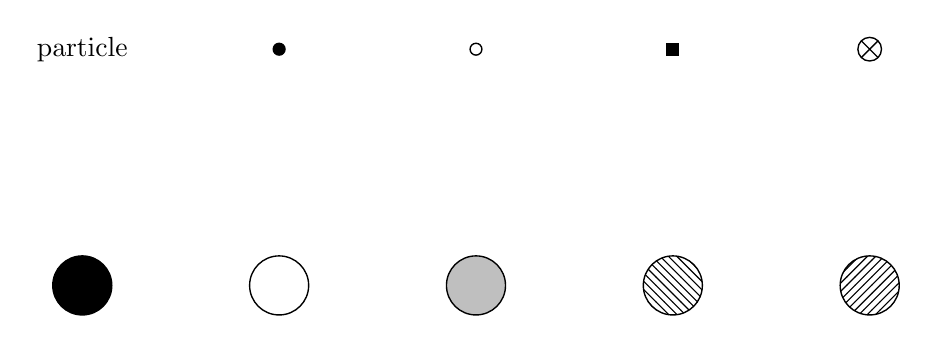
\begin{tikzpicture}  
\begin{feynhand}
  \vertex [particle] (A) at (-5,2) {particle};
  \vertex [dot] (B) at (-2.5,2) {};
  \vertex [ringdot] (C) at (0,2) {};
  \vertex [squaredot] (D) at (2.5,2) {};
  \vertex [crossdot] (E) at (5,2) {};
  \vertex [blob] (F) at (-5,-1) {};
  \vertex [ringblob] (G) at (-2.5,-1) {};
  \vertex [grayblob] (H) at (0,-1) {};
  \vertex [NWblob] (I) at (2.5,-1) {};
  \vertex [NEblob] (J) at (5,-1) {};
\end{feynhand}
\end{tikzpicture} 
\end{figure}
始点,終点には[particle]を用いるのが良い.また,残念ながら電子格子相互作用で用いられる三角バーテックスや,電子間相互作用で用いられる四角バーテックスはない.これはそのうちスタイルファイルを見て,自分で追加するのが良いかもしれない.

\section{伝線}
伝線はpropagコマンドで生成できる.こちらも粒子の種類によってオプションが用意されており
photon, fermion, anti fermion, boson, charged boson, anti charged
boson, gluon, scalar, charged scalar, anti charged scalar, ghost,
charged ghost, anti charged ghost, majorana, anti majorana

\section{sample1}
ここでは一つ$\beta$崩壊のクォークレベルでのダイヤグラムを示す.
\begin{figure}[htb]
\centering
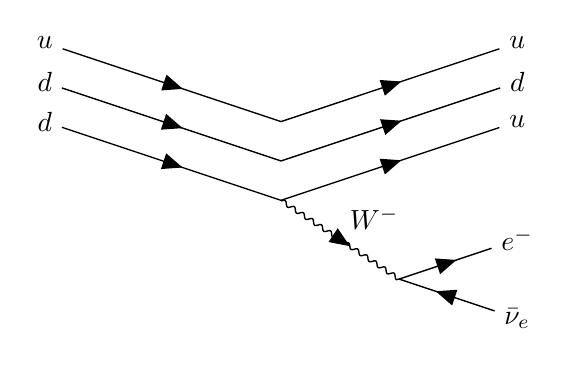
\begin{tikzpicture}
 \begin{feynhand}
 \vertex [particle] (i1) at (-3,4) {$u$};
    \vertex [particle] (i2) at (-3,3.5) {$d$};
    \vertex [particle] (i3) at (-3,3) {$d$};
    \vertex [particle] (f1) at (3,4) {$u$};
    \vertex [particle] (f2) at (3,3.5) {$d$};
    \vertex [particle] (f3) at (3,3) {$u$};
    \vertex (w1) at (0,3);  
    \vertex (w2) at (0,2.5);
    \vertex (w3) at (0,2);
    \vertex (w4) at (1.5,1);
    \vertex [particle] (e) at (3,1.5) {$e^{-}$};
    \vertex [particle] (an) at (3,0.5) {$\bar{\nu}_{e}$};
   \propag [fermion] (i1) to (w1);
   \propag [fermion] (i2) to (w2);
   \propag [fermion] (i3) to (w3);
   \propag [fermion] (w1) to (f1);
   \propag [fermion] (w2) to (f2);
   \propag [fermion] (w3) to (f3);
   \propag [charged boson] (w3) to [edge label=$W^{-}$] (w4);
   \propag [fermion] (w4) to (e);
   \propag [anti fermion] (w4) to (an);
 \end{feynhand}
\end{tikzpicture}
\caption{$\beta$崩壊のダイヤグラム}
\label{213442_4Aug19}
\end{figure}


\section{電子格子相互作用のダイヤグラム}
次に電子とフォノンが相互作用する一次のダイヤグラムを書く.フォノン線として[boson]を用いることにしよう.しばしば後述のクーロン相互作用に用いる[scaler]と逆の表記を用いている文献もあることに注意しよう.
\begin{figure}[htb]
 \centering
\begin{tikzpicture}
\begin{feynhand}
 \vertex [dot] (A) at (0,0) {$g$};
 \vertex [particle] (out) at (-1.5,2) {};
 \vertex [particle] (in)  at (-1.5,-2) {}; 
 \vertex [particle] (phonon) at (3,0) {};
\propag [fermion] (A) to (out);
\propag [fermion] (in) to (A);
\propag [boson]   (A) to (phonon);
\end{feynhand}
\end{tikzpicture}
\caption{電子フォノン相互作用の$1$次}
\end{figure}

\section{電子格子交互作用の$2$次}
電子格子の$2$次の相互作用はよく見かける.
\begin{figure}[htb]
 \centering
\begin{tikzpicture}
 \begin{feynhand}
  %vertex
  \vertex [dot] (v1) at (0,0) {};
  \vertex [dot] (v2) at (3,0) {};
  \vertex [particle] (out1) at (-1.5,2) {};
  \vertex [particle] (in1)  at (-1.5,-2) {}; 
  \vertex [particle] (out2) at (4.5,2) {};
  \vertex [particle] (in2)  at (4.5,-2) {};  
  %propagator
  \propag [fermion] (v1) to (out1);
  \propag [fermion] (in1) to (v1);
  \propag [boson]   (v1) to (v2);
  \propag [fermion] (v2) to (out2);
  \propag [fermion] (in2) to (v2);
 \end{feynhand}
\end{tikzpicture}
\caption{電子フォノン相互作用の$2$次のダイヤグラム}
\end{figure}

\section{クーロン相互作用}
クーロン相互作用にはscalerを用いる.例えば二次の相互作用は単にフォノン線をスカラー線で置き換えれば良いから,
\begin{figure}[htb]
 \centering
\begin{tikzpicture}
 \begin{feynhand}
  %vertex
  \vertex [dot] (v1) at (0,0) {};
  \vertex [dot] (v2) at (3,0) {};
  \vertex [particle] (out1) at (-1.5,2) {};
  \vertex [particle] (in1)  at (-1.5,-2) {}; 
  \vertex [particle] (out2) at (4.5,2) {};
  \vertex [particle] (in2)  at (4.5,-2) {};  
  %propagator
  \propag [fermion] (v1) to (out1);
  \propag [fermion] (in1) to (v1);
  \propag [scalar]   (v1) to (v2);
  \propag [fermion] (v2) to (out2);
  \propag [fermion] (in2) to (v2);
 \end{feynhand}
\end{tikzpicture}
\caption{電子間相互作用の$1$次のダイヤグラム}
\end{figure}

\section{ハートリーフォック}
さて,ここまで来て気になるのがグリーン関数や自己エネルギー,分極関数の表現である.これらでは曲がったプロパゲータを書かないといけない.これらはpropagに対するオプションin,outやhalf left,half rightを用いることで使うことができる.

\begin{figure}[htb]
 \centering
 \begin{tikzpicture}
  \begin{feynhand}
   %vertex
   \vertex [dot] (in) at  (0,0) {};
   \vertex [dot] (out) at (3,0) {};
   %propagator
   \propag [fermion] (in) to (out);
   \propag [scalar] (in) to [in=90, out=90,looseness=1.5] (out);
  \end{feynhand}
 \end{tikzpicture}
\caption{フォック項のダイヤグラム}
\end{figure}
オプションloosenessで曲がり具合(楕円の半径)を指定することができる.従って円にしたかったら直線距離の半分を指定してあげれば良いことになる.

フォック項は良くても問題はハートリー項である.ハートリー項のように同じバーテックスに出入りする場合を愚直にやろうとすると図のようになってしまい失敗する.これはtikz-feynhandの限界の一つで,残念ながら正攻法で綺麗に書くことはできないように思う.
\begin{figure}[htb]
 \centering
 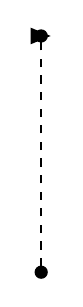
\begin{tikzpicture}
  \begin{feynhand}
   %vertex
   \vertex [dot] (in) at  (0,0) {};
   \vertex [dot] (out) at (0,3) {};
   %propagator
   \propag [scalar] (in) to (out);
   \propag [fermion] (out) to [in=0, out=180,looseness=1.5] (out);
  \end{feynhand}
 \end{tikzpicture}
\caption{ハートリー項のダイヤグラム失敗バージョン}
\end{figure}

そこで少しせこいが,架空のバーテックスを一つ追加してやることで一応,書くことはできる.

\begin{figure}[htb]
 \centering
 \begin{tikzpicture}
  \begin{feynhand}
   %vertex
   \vertex [dot] (in) at  (0,0) {};
   \vertex [dot] (out) at (0,3) {};
   \vertex [particle] (vertial) at (0,6) ;

   %propagator
   \propag [scalar] (in) to (out);
   \propag [fermion] (out) to [in=0, out=0,looseness=1.5] (vertial);
   \propag [fermion] (vertial) to [in=180, out=180,looseness=1.5] (out);

  \end{feynhand}
 \end{tikzpicture}
\caption{ハートリー項のダイヤグラム?}
\end{figure}
ただしこれはあまり良くない例であろうから,ハートリー項のダイヤグラムが欲しければfeynmpを使うことになるだろう.


\section{バブル}
フォック項と同じ要領で例えばRPAのバブルダイヤグラムを書くことができる.

\begin{figure}[htb]
 \centering
 \begin{tikzpicture}
  \begin{feynhand}
   %vertex
   \vertex [dot] (in) at  (0,0) {};
   \vertex [dot] (out1) at (3,0) {};
   \vertex [dot] (out2) at (6,0) {};
   \vertex [dot] (out3) at (9,0) {};
   \vertex [dot] (out4) at (12,0) {};
   %propagator
   \propag [fermion] (in) to [in=90,out=90](out1);
   \propag [fermion] (in) to [in=270, out=270] (out1);
   \propag [scalar] (out1) to (out2);
   \propag [fermion] (out2) to [in=90,out=90](out3);
   \propag [fermion] (out2) to [in=270, out=270] (out3);
   \propag [scalar] (out3) to (out4);
  \end{feynhand}
 \end{tikzpicture}
\caption{RPAのダイヤグラム}
\end{figure}

\end{document}